% !TeX root = ../../thesis.tex

A Bayesian network with structure and parameters learned from the training dataset reached an average Area Under the Receiver Operating Characteristic Curve of 0.857. The results are in the table \ref{tab:result_auc}.

\begin{table}[htpb]
 \caption{Repeated Cross-Validation (10x2) Results: Column description with AUROC along with 95\% CI.} \label{tab:result_auc} 

\renewcommand{\arraystretch}{1.2}
%\setlength{\tabcolsep}{8pt}
\centering
\begin{tabular} { p{1.5cm} p{1.5cm} p{3cm} p{1.5cm} p{1.5cm} l }
\hline
AP & 0.944 & [0.943, 0.945] & VNH & 0.894 & [0.893, 0.895] \\
AG & 0.797 & [0.778, 0.816] & TPEE & 0.816 & [0.815, 0.816] \\
EA & 0.969 & [0.968, 0.969] & AA & 0.751 & [0.743, 0.758] \\
CA & 0.958 & [0.958, 0.958] & GR & 0.931 & [0.93, 0.932] \\
IA & 0.638 & [0.637, 0.638] & V & 0.983 & [0.982, 0.983] \\
PI & 0.881 & [0.88, 0.881] & TP & 0.866 & [0.865, 0.868] \\
IMC & 0.881 & [0.881, 0.882] & VCS & 0.79 & [0.789, 0.791] \\
NRC & 0.75 & [0.75, 0.75] & ANP & 0.942 & [0.938, 0.946] \\
IGA & 0.968 & [0.968, 0.969] & GS & 0.514 & [0.507, 0.52] \\
SGP & 0.974 & [0.974, 0.974] & S & 0.896 & [0.896, 0.897] \\
VA & 0.974 & [0.974, 0.974] & VP & 0.771 & [0.77, 0.772] \\
TG & 0.728 & [0.726, 0.73] & TPNP & 0.952 & [0.951, 0.952] \\
\hline
 \multicolumn{6}{c}{\textbf{Average}  \textbf{0.857 [0.846, 0.868]}} \\

\hline
\end{tabular}
\end{table}


The network is as represented in figure \ref{fig:network}.
%TC:ignore
\begin{figure}[htbp]
\centering
\caption{Bayesian Network learned. Nodes acronyms are explained in appendix 1. The example shows the inference for the Robson Group (10 groups) and the probability of each, given a set of other features. It can be updated with new information (when we know the variables) or leave it empty when unknown. The plausability is calculated comparing the most probable one and the real one. Performance shown in table 2.}\label{fig:network} 
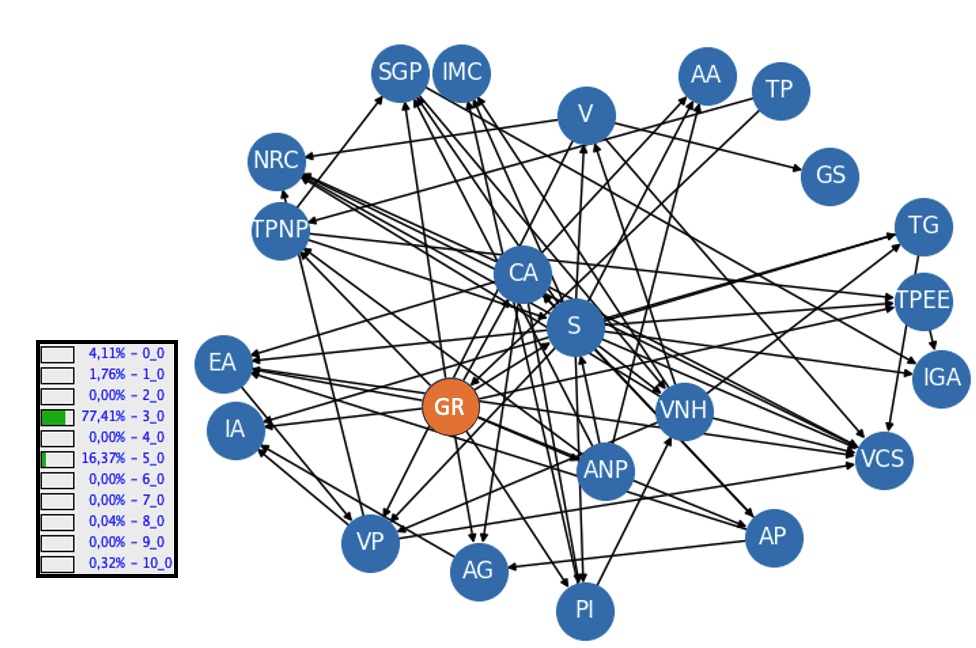
\includegraphics[scale=0.38]{figures/new-bn.png}
\end{figure}
%TC:endignore



\subsection{Deployment \& Validation}

The purpose of this model is to serve as an API for usage within a healthcare institution and act as a supplementary data quality assessment tool. Although a concrete, vendor-specific information model and health information system were initially used, our goal is to develop a more universal clinical decision support system. This system should be usable across all systems involved in birth and obstetrics departments. Therefore, we constructed it using the Health Level 7 (HL7) Fast Healthcare Interoperable Resources (FHIR) R5 version standard. This approach simplifies the process of API interaction. Rather than utilizing a proprietary model for the data, we based our decision on the use of FHIR resources: Bundle and Observation. These resources handle the request and response through a customized operation named "\$quality\_check". We intend to publish the profiles of these objects to streamline API access via standardized mechanisms and data models. The model then makes use of the customized operation and of several base resources to construct a FHIR message, which are: Bundle, MessageHeader, Observation, Device. Observation is where the information about the record is contained, Device contains information about the model, and MessageHeader is used to add information about the request. Finally, the Bundle is used to group all of these resources together. The current version of the profiles can be accessed here\unskip~\cite{obs-ig}. 

For validation, we deployed the tool in docker format in a hospital to gather new data. We gathered 3223 new cases and returned a score for quality as exemplified in figure \ref{fig:scores}. Being that the score is from 0 to 1, the average score was 0.75 and IQR was 0.016. The formula gives weights to different dimensions since we feel some are more robust than others. We gave more weight to rule system, and gave less to the missing and IQR score.

As for the clinicians' assessment, we got 4 answers. Figure \ref{fig:clinical-dq} shows the distribution of the perceived ranking of each record.


%TC:ignore
\begin{figure}[htbp]
\centering
\caption{Model score for newly seen data}\label{fig:scores} 
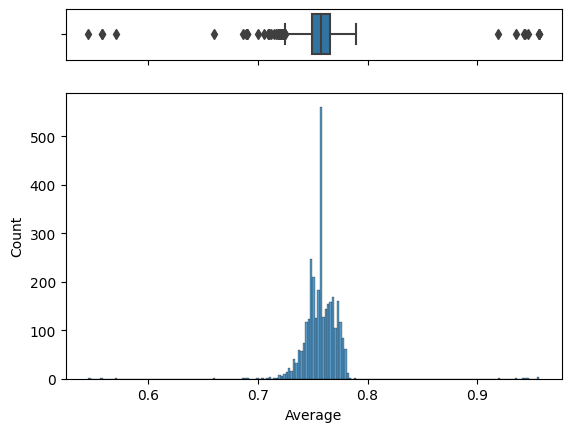
\includegraphics[scale=0.78]{figures/Scoring_V2.png}
\end{figure}
%TC:endignore

%TC:ignore
\begin{figure}[htbp]
\centering
\caption{Distribution of rankings obtained from the assessment of 10 records by 4 different clinicians. Y is the distribution of clinicians' assessment, X is the patient ID.}\label{fig:clinical-dq} 
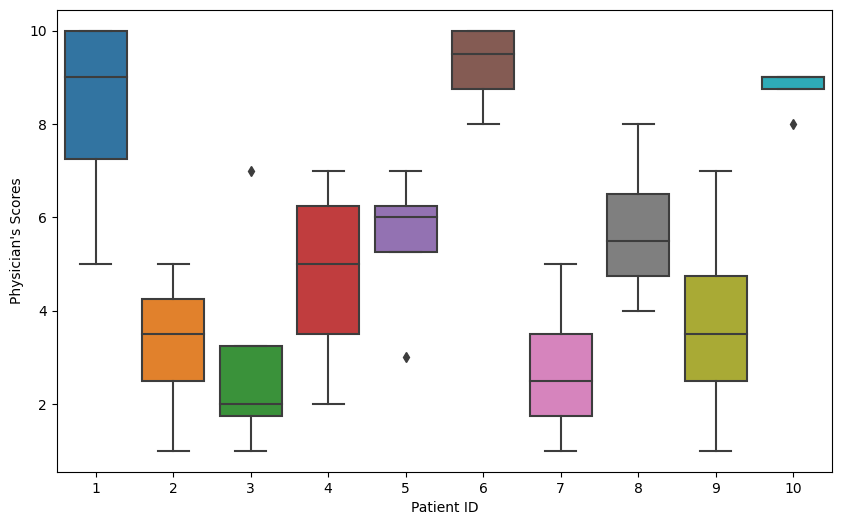
\includegraphics[scale=0.52]{figures/clinical_assessment_no_model.png}
\end{figure}
%TC:endignore

%The Average Spearman's Rank Correlation Coefficient was 0.14 and the Kendall's Tau was 0.096 with a \textit{p-value} of 0.712.
Figure \ref{fig:auc_changes} shows the performance of the model with several ranking thresholds to differentiate bad quality record from good quality record. Each line/color is a threshold (3,4,5,6) and the AUC is shown in the label. The Average Spearman's Rank Correlation Coefficient was 0.42 (p-value: 0.23) and the Kendall's Tau was 0.3 (p-value: 0.2). Both tests were based on a $\alpha$ of 0.05.

%TC:ignore
\begin{figure}[htbp]
    \centering
    \caption{Model Performance in terms of AUROC, depending on the threshold defined on the physician assessed data. The colors show different threshold used to consider a bad quality record given the average ranking. Label shows the threshold and respective AUROC.}\label{fig:auc_changes} 
    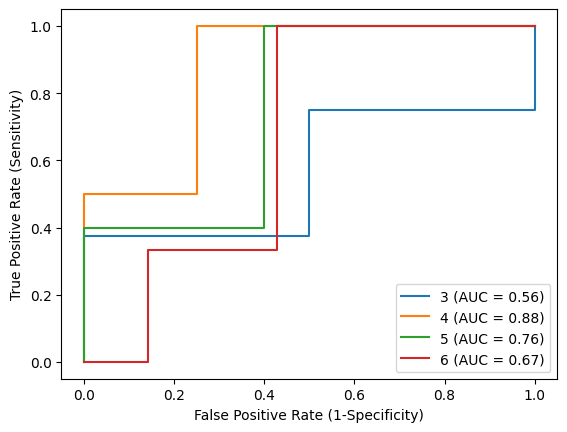
\includegraphics[scale=0.78]{figures/auroc_curve_threshold.png}
    \end{figure}
    %TC:endignore